% XeLaTeX can use any Mac OS X font. See the setromanfont command below.
% Input to XeLaTeX is full Unicode, so Unicode characters can be typed directly into the source.

% The next lines tell TeXShop to typeset with xelatex, and to open and save the source with Unicode encoding.

%!TEX TS-program = xelatex
%!TEX encoding = UTF-8 Unicode

\documentclass[11pt,twoside,openany]{book}
\usepackage{multirow}
\usepackage{pdfpages}

\usepackage{xspace}

\usepackage{array}
\usepackage{lipsum}

\usepackage{algorithm}
\usepackage{algpseudocode}

\usepackage{geometry}                % See geometry.pdf to learn the layout options. There are lots.
%\usepackage[margin=1cm]{geometry}


% \addtolength{\textwidth}{1.75in}
%
% \addtolength{\topmargin}{-.875in}
% \addtolength{\textheight}{1.75in}

\geometry{a4paper,left=20mm,top=20mm,bottom=50mm,total={162mm,230mm}}                   % ... or a4paper or a5paper or ...
%\geometry{landscape}                % Activate for for rotated page geometry
%\usepackage[parfill]{parskip}    % Activate to begin paragraphs with an empty line rather than an indent
\usepackage{amssymb}
%\usepackage{todonotes}
\setlength{\marginparwidth}{2cm}
\usepackage[backgroundcolor=white,bordercolor=blue,linecolor=blue,textwidth=1cm]{todonotes}
\usepackage{booktabs}
\usepackage{longtable}
\usepackage{url}

\usepackage[depth=4]{bookmark}


\usepackage{algorithm}
\usepackage{algpseudocode}

\usepackage{imakeidx}
\usepackage[utf8]{inputenc}
\usepackage[T1]{fontenc}
\makeindex[intoc]

\usepackage[font=normalsize]{caption}

\renewcommand{\theparagraph}{\S\arabic{paragraph}}
\setcounter{secnumdepth}{4}


\usepackage{xcolor}
\usepackage{listings}

\makeatletter
\global\let\tikz@ensure@dollar@catcode=\relax
\makeatother

\definecolor{mGreen}{rgb}{0,0.6,0}
\definecolor{mGray}{rgb}{0.5,0.5,0.5}
\definecolor{mPurple}{rgb}{0.58,0,0.82}
\definecolor{backgroundColour}{rgb}{0.95,0.95,0.92}
\definecolor{gray}{rgb}{0.4,0.4,0.4}
\definecolor{darkblue}{rgb}{0.0,0.0,0.6}
\definecolor{cyan}{rgb}{0.0,0.6,0.6}

\lstdefinestyle{CStyle}{
    backgroundcolor=\color{backgroundColour},
    commentstyle=\color{mGreen},
    keywordstyle=\color{magenta},
    numberstyle=\tiny\color{mGray},
    stringstyle=\color{mPurple},
    basicstyle=\scriptsize\ttfamily,
    breakatwhitespace=false,
    breaklines=true,
    captionpos=b,
    keepspaces=true,
    numbers=left,
    numbersep=5pt,
    showspaces=false,
    showstringspaces=false,
    showtabs=false,
    tabsize=2,
    language=C
}


\lstset{
  backgroundcolor=\color{white},   % choose the background color; you must add \usepackage{color} or \usepackage{xcolor}; should come as last argument
  basicstyle=\footnotesize\ttfamily,        % the size of the fonts that are used for the code
  breakatwhitespace=false,         % sets if automatic breaks should only happen at whitespace
  breaklines=true,                 % sets automatic line breaking
  captionpos=b,                    % sets the caption-position to bottom
  commentstyle=\color{gray},    % comment style
  deletekeywords={...},            % if you want to delete keywords from the given language
  %escapeinside={\%*}{*)},          % if you want to add LaTeX within your code
  %extendedchars=true,              % lets you use non-ASCII characters; for 8-bits encodings only, does not work with UTF-8
  %firstnumber=1000,                % start line enumeration with line 1000
  frame=single,                    % adds a frame around the code
  keepspaces=true,                 % keeps spaces in text, useful for keeping indentation of code (possibly needs columns=flexible)
  keywordstyle=\color{blue},       % keyword style
  language=C,                 % the language of the code
  %morekeywords={*,...},            % if you want to add more keywords to the set
  numbers=left,                    % where to put the line-numbers; possible values are (none, left, right)
  numbersep=5pt,                   % how far the line-numbers are from the code
  numberstyle=\tiny\color{gray}, % the style that is used for the line-numbers
  rulecolor=\color{black},         % if not set, the frame-color may be changed on line-breaks within not-black text (e.g. comments (green here))
  showspaces=false,                % show spaces everywhere adding particular underscores; it overrides 'showstringspaces'
  showstringspaces=false,          % underline spaces within strings only
  showtabs=false,                  % show tabs within strings adding particular underscores
  stepnumber=1,                    % the step between two line-numbers. If it's 1, each line will be numbered
  stringstyle=\color{black},     % string literal style
  tabsize=2,                     % sets default tabsize to 2 spaces
}

\lstset{
  columns=fullflexible,
  showstringspaces=false,
  commentstyle=\color{gray}\upshape,
  backgroundcolor=\color{backgroundColour},
  commentstyle=\color{mGreen},
  keywordstyle=\color{magenta},
  numberstyle=\tiny\color{mGray},
  stringstyle=\color{mPurple},
  basicstyle=\scriptsize\ttfamily,
  tabsize=2
}

\lstdefinelanguage{XML}
{
  morestring=[b]",
  morestring=[s]{>}{<},
  morecomment=[s]{<?}{?>},
  stringstyle=\color{black},
  identifierstyle=\color{darkblue},
  keywordstyle=\color{cyan},
  morekeywords={xmlns,version,type}% list your attributes here
}


% Will Robertson's fontspec.sty can be used to simplify font choices.
% To experiment, open /Applications/Font Book to examine the fonts provided on Mac OS X,
% and change "Hoefler Text" to any of these choices.

\usepackage{fontspec,xltxtra,xunicode}
\defaultfontfeatures{Mapping=tex-text}
\setromanfont[Mapping=tex-text]{Optima}
\setsansfont[Scale=MatchLowercase,Mapping=tex-text]{Optima}
\setmonofont[Scale=MatchLowercase]{Andale Mono}

%%%% Graphics
\usepackage{graphicx}
\usepackage{tikz}
\definecolor{unilublue}{RGB}{55,149,218}
\definecolor{sntred}{RGB}{219,46,27}
\definecolor{sntpurple}{RGB}{86,30,130}
%\definecolor{sntblue}{RGB}{50,130,207}
\definecolor{sntblue}{RGB}{55,149,218}

\pgfdeclareimage[width=30mm]{logo-snt}{logos/logo-snt}
\pgfdeclareimage[width=30mm]{logo-uni-lu}{logos/logo-uni-lu}

%%%% Fancy
\usepackage{fancyhdr}

%%%% Increase page length
\addtolength{\textheight}{1in}

%%%% Sections
\usepackage{sectsty}
\allsectionsfont{\sffamily}

\setlength{\parskip}{1em}

%\renewcommand{\,}{$^{\cdot}$}

\usepackage{hyperref}
\hypersetup{
    colorlinks,
    citecolor=black,
    filecolor=black,
    linkcolor=black,
    urlcolor=black
}


%%%% Title
\newcommand{\titleone}{\textsf{FAQAS Framework}}
\newcommand{\titletwo}{\textsf{SUTR}}
\newcommand{\titlethree}{\textsf{Software Unit Test Report}}

\newcommand{\todoinline}[1]{\todo[color=orange,inline]{ \textbf{TODO}: #1 }}

\newcommand{\TODO}[1]{\todo[color=orange,inline]{ \textbf{TODO}: #1 }}
\newcommand{\OSCAR}[1]{\todo[color=yellow,inline]{ \textbf{OSCAR}: #1 }}
\newcommand{\DONE}[1]{\todo[color=green,inline]{ \textbf{DONE}: #1 }}

\newcommand{\CHANGEDTWO}[1]{\textcolor{black}{#1}}

\newcommand{\EMPH}[1]{\textbf{\emph{#1}}}
\newcommand{\INDEX}[1]{\index{\MakeLowercase{#1}}\EMPH{#1}}

\newcommand{\MASS}{\textit{MASS}\xspace{}}

\newcommand{\DAMA}{\textit{DAMAt}\xspace{}}

\newcounter{paranum}
\newcommand{\RQ}{\vspace{10pt}\noindent\textbf{FAQAS-SSS-REQ-\refstepcounter{paranum}\ifnum\value{paranum}<10 00\else 0\fi\theparanum}\textbf}

\newcommand{\remark}{\textbf{Remark:}\xspace}

\begin{document}

\pagestyle{fancy}
\renewcommand{\sectionmark}[1]{\markright{\textit{#1}}}

\renewcommand{\headrulewidth}{2pt}% 2pt header rule
\renewcommand{\headrule}{\hbox to\headwidth{%
  \color{sntblue}\leaders\hrule height \headrulewidth\hfill}}

\fancyhf{}

%\lhead{\fancyplain{}{\setlength{\unitlength}{1mm}
%\begin{picture}(0,0)
%\put(0,-4){
\includegraphics[width=50pt]{logos/logo-snt}}
%\end{picture}}}

\newcommand{\DOCUMENTID}{ITT-1-9873-ESA-FAQAS-SUTR}
\lhead{\fancyplain{}{\textit{\DOCUMENTID}}}
\rhead{\fancyplain{}{\rightmark }}


\fancyfoot[C]{%
\begin{tikzpicture}[remember picture,overlay]
\path [fill=sntred]    ([xshift=88pt,yshift=20pt]current page.south west) rectangle
                       ([xshift=229pt,yshift=50pt] current page.south west);
\path [fill=sntpurple] ([xshift=229pt,yshift=20pt] current page.south west) rectangle
                       ([xshift=370pt,yshift=50pt] current page.south west);
\path [fill=sntblue]   ([xshift=370pt,yshift=20pt] current page.south west) rectangle
                       ([xshift=510pt,yshift=50pt] current page.south west);
\end{tikzpicture}
}

\fancyfoot[RO]{
\begin{tikzpicture}[remember picture,overlay]
\node [circle, ultra thick, fill=white, draw=sntblue] at ([xshift=530pt,yshift=35pt] current page.south west) {\thepage};
\end{tikzpicture}}

\fancyfoot[LE]{
\begin{tikzpicture}[remember picture,overlay]
\node [circle, ultra thick, fill=white, draw=sntblue] at ([xshift=65pt,yshift=35pt] current page.south west) {\thepage};
\end{tikzpicture}}


\newcommand{\STARTCHANGEDWPT}{\color{black}}
\newcommand{\ENDCHANGEDWPT}{\color{black}}

\newcommand{\STARTCHANGEDFR}{\color{blue}}
\newcommand{\ENDCHANGEDFR}{\color{black}}


\newcommand{\CHANGED}[1]{{#1}}
\newcommand{\prog}{P}
\newcommand{\prop}{}

\newcommand{\FAQAS}{FAQAS-framework\xspace}


\newcommand{\REVISION}[2]{{#2}}
\newcommand{\REVTOOL}[2]{\todo{\tiny{#1}}\color{blue}{#2}\color{black}}

\newcommand{\REVTWO}[2]{#2}

\thispagestyle{empty}

\begin{tikzpicture}[remember picture,overlay]
\path [fill=sntred]    ([xshift=30pt,yshift=20pt]current page.south west) rectangle
                       ([xshift=210pt,yshift=50pt] current page.south west);
\path [fill=sntpurple] ([xshift=210pt,yshift=20pt] current page.south west) rectangle
                       ([xshift=390pt,yshift=50pt] current page.south west);
\path [fill=sntblue]   ([xshift=390pt,yshift=20pt] current page.south west) rectangle
                       ([xshift=570pt,yshift=51pt] current page.south west);
\path [fill=unilublue] ([xshift=30pt,yshift= 50pt] current page.south west) --
                       ([xshift=570pt,yshift= 50pt] current page.south west)
                       [rounded corners=20pt] --
                       ([xshift=570pt,yshift=740pt] current page.south west)
                       [sharp corners] --
                       ([xshift=30pt,yshift=740pt] current page.south west);
\node [fill=white,rounded corners=0pt,inner xsep=6pt,inner ysep=3pt]
      at ([xshift=523pt,yshift=120pt] current page.south west)
      {\pgfuseimage{logo-uni-lu}};

\node [fill=white,rounded corners=2pt,inner xsep=6pt,inner ysep=3pt]
      at ([xshift=520pt,yshift=780pt] current page.south west)
      {\pgfuseimage{logo-snt}};

%\node [circle, fill=white, draw=sntblue] at ([xshift=550pt,yshift=35pt] current page.south west) {a};

\node[draw=none,fill=none,right] at (-1, -7){\color{white}\LARGE\bf\titleone};
\node[draw=none,fill=none,right] at (-1, -8){\color{white}\LARGE\bf\titletwo};
\node[draw=none,fill=none,right] at (-1, -9){\color{white}\LARGE\bf\titlethree};

\node[draw=none,fill=none,right] at (-1, -12){\color{white}\Large\textsf{O. Cornejo, F. Pastore, E. Viganò}};
\node[draw=none,fill=none,right] at (-1, -13){\color{white}\Large\textsf{Interdisciplinary Centre for Security, Reliability and Trust}};
\node[draw=none,fill=none,right] at (-1, -14){\color{white}\Large\textsf{University of Luxembourg}};
\node[draw=none,fill=none,right] at (11, -16){\color{white}\textsf{ITT-1-9873-ESA-FAQAS-SUTP}};
\node[draw=none,fill=none,right] at (11, -17){\color{white}\Large\textsf{Issue 4, Rev. 1}};
\node[draw=none,fill=none,right] at (11, -18){\color{white}\Large\textsf{\today}};
\node[draw=none,fill=none,right] at (-1, -24){\color{white}\tiny\textsf{EUROPEAN SPACE AGENCY. CONTRACT REPORT.}};
\node[draw=none,fill=none,right] at (-1, -24.3){\color{white}\tiny\textsf{The work described in this report was done under ESA contract. Responsibility for the contents resides in the author or organisation that prepared it.}};
\node[draw=none,fill=none,right] at (-1, -24.8){\color{white}\tiny\textsf{The copyright in this document is vested in the University of Luxembourg.}};
\node[draw=none,fill=none,right] at (-1, -25.1){\color{white}\tiny\textsf{This document may only be reproduced in whole or in part, or stored in a retrieval system,or transmitted in any form, or by any means electronic,}};
\node[draw=none,fill=none,right] at (-1, -25.4){\color{white}\tiny\textsf{mechanical, photocopying or otherwise, either with the prior permission of the University of Luxembourg or in accordance with the terms of ESTEC Contract No. 4000128969/19/NL/AS.}};

\node[draw=none,fill=none,right] at (-1, -24){\color{white}\tiny\textsf{EUROPEAN SPACE AGENCY. CONTRACT REPORT.}}; 
\node[draw=none,fill=none,right] at (-1, -24.3){\color{white}\tiny\textsf{The work described in this report was done under ESA contract. Responsibility for the contents resides in the author or organisation that prepared it.}};
\node[draw=none,fill=none,right] at (-1, -24.8){\color{white}\tiny\textsf{The copyright in this document is vested in the University of Luxembourg.}};
\node[draw=none,fill=none,right] at (-1, -25.1){\color{white}\tiny\textsf{This document may only be reproduced in whole or in part, or stored in a retrieval system,or transmitted in any form, or by any means electronic,}}; 
\node[draw=none,fill=none,right] at (-1, -25.4){\color{white}\tiny\textsf{mechanical, photocopying or otherwise, either with the prior permission of the University of Luxembourg or in accordance with the terms of ESTEC Contract No. 4000128969/19/NL/AS.}};


\end{tikzpicture}

\newpage


% !TEX root = MAIN.tex

\section*{Revisions}
\label{sec:revisions}


\setlength\LTleft{0pt}
\setlength\LTright{0pt}
\tiny 
%@{\extracolsep{\fill}}
\begin{longtable}{|p{2cm}|p{1cm}|p{1.5cm}|p{9cm}|@{}}
\label{table:codeoperators} \\
\hline
\textbf{Issue Number}&\textbf{Date}&\textbf{Authors}&\textbf{Description}\\
\hline
ITT-1-9873-ESA-FAQAS-FR
Issue 1 Rev. 1&
October 29th, 2021&
Fabrizio Pastore, Oscar Cornejo, Enrico Viganò&
\begin{minipage}{8cm}
Initial release.
\end{minipage}
\\
\hline
ITT-1-9873-ESA-FAQAS-FR
Issue 1 Rev. 2&
November 11th, 2021&
Fabrizio Pastore, Oscar Cornejo, Enrico Viganò&
\begin{minipage}{8cm}
Added Chapter~\ref{chap:deliverables_summary} (deliverables summary).\\
Added Chapter~\ref{ch:toolset} (description of toolset package).\\
Added information about input and outputs of the tools in Chapter~\ref{chapter:methodology} (see blue text).
\end{minipage}
\\
\hline
                                                    
\end{longtable}
\normalsize

\clearpage


\tableofcontents


% !TEX root = MAIN.tex

\chapter{Scope and content}

This document is the deliverable SSS of the ESA activity ITT-1-9873-ESA. It concerns requirements specification for the \emph{FAQAS framework} to be delivered by ITT-1-9873-ESA. Following the structure described in the SoW \emph{AO9873-ws00pe\_SOW.pdf}, it provides the structured requirements baseline for the FAQAS framework according to ECSS-E-ST-40C Annex B.
 
\section{Applicable and reference documents}

\begin{itemize}
\item{D1 - Mutation testing survey}
\item{D2 - Study of mutation testing applicability to space software}
\end{itemize}

\chapter{Terms, definitions and abbreviated terms}

\begin{itemize}
\item{FAQAS}: activity ITT-1-9873-ESA
\item{FAQAS-framework}: software system to be released at the end of WP4 of FAQAS
\item{D2}: Deliverable D2 of FAQAS, \emph{Study of mutation testing applicability to space software}
\item{KLEE}: Third party test generation tool, details are provided in D2.
\item{SUT}: Software under test, i.e, the software that should be mutated by means of mutation testing.
\item{WP}: Work package
\end{itemize}

\clearpage
 



% !TEX root = MAIN.tex

\chapter{\MASS{} - Unit Test Execution Environment Definition}

One unit test procedure was identified for \MASS:
\begin{itemize}
  \item {\emph{MASS-TD-SRCMutation-1}} that targets the unit \emph{SRCMutation}.
\end{itemize}

These unit test procedures are defined in the \emph{SUITP}.

The testing environment is described below:

\begin{center}
\begin{tabular}{ |c|c| }
 \hline
 Platform & Ubuntu 18.04.3 LTS (Bionic Beaver) 4.15.0-58-generic \\
 \hline
 Toolchain & GCC 7.5.0 \\
 \hline
 Python version & Python 3.6.9 \\
 \hline
 Bash version & GNU bash, version 4.4.20(1)-release (x86\_64-pc-linux-gnu) \\
 \hline
\end{tabular}
\end{center}


\chapter{\MASS{} - 1.0 - Result Summary}

\REVTOOL{P-C-05}{\textbf{Version under test}: 1.0}

A summary of the results of the test suite as of Monday 20/09/2021 is present in the following in tabular form.
For every test case the following information are available:
\begin{itemize}
  \item Operator
  \item Term to replace
  \item Replacements
  \item Test case
  \item Result
\end{itemize}

The definition and configuration of the test cases are reported in the \emph{SUTP}.

Test logs had been uploaded to Alfresco, with name \texttt{SUTR-Logs-MASS-2021\_09\_20.zip}.

\section{\MASS - MASS-TD-SRCMutation-1}

% !TEX root =  ../MAIN.tex

\setlength\LTleft{0pt}
\setlength\LTright{0pt}
\scriptsize
\begin{longtable}{|p{1cm}|p{5cm}|p{6cm}|p{2.5cm}|}

% \begin{table}[h]
% \scriptsize
% \centering
\caption{Unit test cases for SRCMutation.}
\label{table:matrix} \\

% \begin{tabular}{|llp{6cm}l|}
\hline 
\textbf{Operator}	&	\textbf{Term to replace}	&	\textbf{Replacements}	&	\textbf{Test Case} \\
\hline 
ABS	&	$a$	&	$-a$	&	abs\_val.sh \\
ABS	&	$a,b$	&	$-a,-b$	&	abs\_many.sh \\
AOR	&	$+$	&	$\{-,*,/,\%\}$	&	aor\_plus.sh \\
AOR	&	$-$	&	$\{+,*,/,\%\}$	&	aor\_minus.sh \\
AOR	&	$*$	&	$\{+,-,/,\%\}$	&	aor\_mult.sh \\
AOR	&	$/$	&	$\{+,-,*,\%\}$	&	aor\_div.sh \\
AOR	&	$\%$	&	$\{+,-,*,/\}$	&	aor\_mod.sh \\
AOR	&	$+=$	&	$\{-=,*=,/=,\%=\}$	&	aor\_plus\_assign.sh \\
AOR	&	$-=$	&	$\{+=,*=,/=,\%=\}$	&	aor\_minus\_assign.sh \\
AOR	&	$*=$	&	$\{+=,-=,/=,\%=\}$	&	aor\_mult\_assign.sh \\
AOR	&	$/=$	&	$\{+=,-=,*=,\%=\}$	&	aor\_div\_assign.sh \\
AOR	&	$\%=$	&	$\{+=,-=,*=,/=\}$	&	aor\_mod\_assign.sh \\
AOR	&	$+,-$	&	$\{+,-,*,\%\}$	&	aor\_many.sh \\
ICR	&	$10$	&	$\{1, -1, 0, 11, 9, -10\}$	&	icr\_val.sh \\
ICR	&	$10 + 1$	&	$\{1+1, -1+1, 10-1, 0+1, 10+0, 10+1, 10+2, 10-1+1, -10+1\}$	&	icr\_many.sh \\
LCR	&	$\&\&$	&	$||$	&	lcr\_logic\_or.sh \\
LCR	&	$||$	&	$\&\&$	&	lcr\_logic\_and.sh \\
LCR	&	$\&$	&	$\{|,\land\}$	&	lcr\_and.sh \\
LCR	&	$|$	&	$\{\&,\land\}$	&	lcr\_or.sh \\
LCR	&	$\land$	&	$\{\&,|\}$	&	lcr\_xor.sh \\
LCR	&	$\&=$	&	$\{|=, \land=\}$	&	lcr\_and\_assign.sh \\
LCR	&	$|=$	&	$\{\&=, \land=\}$	&	lcr\_or\_assign.sh \\
LCR	&	$\land=$	&	$\{\&=, |=\}$	&	lcr\_xor\_assign.sh \\
LCR	&	$\land, \&\&$	&	$\{\&,|,||\}$	&	lcr\_many.sh \\
ROR	&	$>$	&	$\{>=, <, <=, ==, !=\}$	&	ror\_gt.sh \\
ROR	&	$>=$	&	$\{>, <, <=, ==, !=\}$	&	ror\_ge.sh \\
ROR	&	$<$	&	$\{>, >=, <=, ==, !=\}$	&	ror\_lt.sh \\
ROR	&	$<=$	&	$\{>, >=, <, ==, !=\}$	&	ror\_le.sh \\
ROR	&	$==$	&	$\{>, >=, <, <=, !=\}$	&	ror\_eq.sh \\
ROR	&	$!=$	&	$\{>, >=, <, <=, ==\}$	&	ror\_neq.sh \\
ROR	&	\texttt{if(a)}	&	\texttt{if(!a)}	&	ror\_if.sh \\
ROR	&	\texttt{while(a)}	&	\texttt{while(!a)}	&	ror\_while.sh \\
ROR	&	\texttt{if(a), >}	&	\texttt{if(!a), >=, <, <=, ==, !=}	&	ror\_many.sh \\
SDL	&	\texttt{int a = 0;} &	\texttt{}	&	sdl.sh \\
SDL	&	\texttt{int a = 0; return;} &	\{\texttt{int a = 0;},\texttt{return;}\}	&	sdl\_many.sh \\
UOI	&	$b$	&	$\{\texttt{--}b, b\texttt{--}, \texttt{++}b, b\texttt{++}\}$	&	uoi.sh \\
UOI	&	$a,b$	&	$\{\texttt{--}\{a,b\}, \{a,b\}\texttt{--}, \texttt{++}\{a,b\}, \{a,b\}\texttt{++}\}$	&	uoi\_many.sh \\
AOD	&	$a + b$	&	$\{a, b\}$	&	aod\_plus.sh \\
AOD	&	$a - b$	&	$\{a, b\}$	&	aod\_minus.sh \\
AOD	&	$a * b$	&	$\{a, b\}$	&	aod\_mult.sh \\
AOD	&	$a / b$	&	$\{a, b\}$	&	aod\_div.sh \\
AOD	&	$a \% b$	&	$\{a, b\}$	&	aod\_mod.sh \\
AOD	&	$a / b + 1$	&	\texttt{\{1, b+1, a+1, a/b\}}	&	aod\_many.sh \\
LOD	&	$a > 0 \&\& b > 0$	&	\texttt{\{a > 0, b > 0\}}	&	lod\_logic\_and.sh \\
LOD	&	$a > 0 || b > 0$	&	\texttt{\{a > 0, b > 0\}}	&	lod\_logic\_or.sh \\
LOD	&	$a > 0 \&\& b > 0) || 1$	&	\texttt{\{1, b>0 || 1, a>0 || 1, a>0 \&\& b>0\}}	&	lod\_many.sh \\
ROD	&	$a>b$	&	$\{a, b\}$	&	rod\_gt.sh \\
ROD	&	$a>=b$	&	$\{a, b\}$	&	rod\_ge.sh \\
ROD	&	$a<b$	&	$\{a, b\}$	&	rod\_lt.sh \\
ROD	&	$a<=b$	&	$\{a, b\}$	&	rod\_le.sh \\
ROD	&	$a==b$	&	$\{a, b\}$	&	rod\_eq.sh \\
ROD	&	$a!=b$	&	$\{a, b\}$	&	rod\_neq.sh \\
ROD	&	$a == b \&\& a != 0$	&	\texttt{\{b \&\& a != 0, a == b \&\&  0, a  \&\& a != 0, a == b \&\& a\}}	&	rod\_many.sh \\
BOD	&	$a\&b$	&	$\{a, b\}$	&	bod\_and.sh \\
BOD	&	$a|b$	&	$\{a, b\}$	&	bod\_or.sh \\
BOD	&	$a \land b$	&	$\{a, b\}$	&	bod\_xor.sh \\
BOD	&	$a \& b \& 1$	&	\texttt{\{1, b \& 1, a \& 1, a \& b\}}	&	bod\_many.sh \\
SOD	&	$a>>b$	&	$\{a, b\}$	&	sod\_sl.sh \\
SOD	&	$a<<b$	&	$\{a, b\}$	&	sod\_sr.sh \\
SOD	&	$a >> b || b << a$	&	\texttt{\{b || b << a,a >> b || a, a || b << a, a >> b || b\}}	&	sod\_many.sh \\
LVR	&	$0$	&	$-1$	&	lvr\_zero.sh \\
LVR	&	$3.5$	&	$\{-3.5, 0\}$	&	lvr\_literal.sh \\
LVR	&	\texttt{true}	&	\texttt{false}	&	lvr\_true.sh \\
LVR	&	\texttt{false}	&	\texttt{true}	&	lvr\_false.sh \\
LVR	&	\texttt{true \& false}	&	\texttt{false \& false}, \texttt{true \& true}	&	lvr\_many.sh \\
ALL	&	\texttt{int a = 4, b = 5; return a + b;}	&	\texttt{int a = 4, b = 1; return a + b;}	&	many.sh \\
& & \texttt{return a + b;} & \\
& & \texttt{int a = 1, b = 5; return a + b;} & \\
& & \texttt{int a = (-1), b = 5; return a + b;} & \\
& & \texttt{int a = 4, b = (-1); return a + b;} & \\
& & \texttt{int a = 4, b = 0; return a + b;} & \\
& & \texttt{int a = 0, b = 5; return a + b;} & \\
& & \texttt{int a = (4 + 1), b = 5; return a + b;} & \\
& & \texttt{int a = 4, b = (5 + 1); return a + b;} & \\
& & \texttt{int a = (4 - 1), b = 5; return a + b;} & \\
& & \texttt{int a = 4, b = (5 - 1); return a + b;} & \\
& & \texttt{int a = 4, b = -(5); return a + b;} & \\
& & \texttt{int a = -(4), b = 5; return a + b;} & \\
& & \texttt{int a = 4, b = 5;} & \\
& & \texttt{int a = 4, b = 5; return -(a) + b;} & \\
& & \texttt{int a = 4, b = 5; return  b;} & \\
& & \texttt{int a = 4, b = 5; return a + -(b);} & \\
& & \texttt{int a = 4, b = 5; return (--a) + b;} & \\
& & \texttt{int a = 4, b = 5; return a + (--b);} & \\
& & \texttt{int a = 4, b = 5; return a ;} & \\
& & \texttt{int a = 4, b = 5; return a - b;} & \\
& & \texttt{int a = 4, b = 5; return (a--) + b;} & \\
& & \texttt{int a = 4, b = 5; return a + (b--);} & \\
& & \texttt{int a = 4, b = 5; return (++a) + b;} & \\
& & \texttt{int a = 4, b = 5; return a * b;} & \\
& & \texttt{int a = 4, b = 5; return a + (++b);} & \\
& & \texttt{int a = 4, b = 5; return (a++) + b;} & \\
& & \texttt{int a = 4, b = 5; return a / b;} & \\
& & \texttt{int a = 4, b = 5; return a + (b++);} & \\
& & \texttt{int a = 4, b = 5; return a \% b;} & \\
\hline
% \end{tabular}
\end{longtable}
\normalsize


\clearpage


% !TEX root = MAIN.tex

\chapter{\DAMA - Unit Test Execution Environment Definition and Results}

Two unit test procedures were identified for \DAMA:
\begin{itemize}
  \item {\emph{DAMAt-TD-DDMutation-1}} that targets the unit \emph{DDMutationFault}.
  \item {\emph{DAMAt-TD-DDMutation-2}} that targets the unit \emph{DDMutationData}.
\end{itemize}

These unit test procedures are defined in the \emph{SUITP}.

The testing environment is described below:

\begin{center}
\begin{tabular}{ |c|c| }
 \hline
 Platform & Ubuntu 18.04.3 LTS (Bionic Beaver) 4.15.0-58-generic \\
 \hline
 Toolchain & GCC 7.5.0 \\
 \hline
 Python version & Python 3.6.9 \\
 \hline
 Bash version & GNU bash, version 4.4.20(1)-release (x86\_64-pc-linux-gnu) \\
 \hline
 Valgrind version & valgrind-3.13.0 \\
 \hline
\end{tabular}
\end{center}

% \chapter{\DAMA -  Test Suite Software Configuration}

\chapter{\DAMA - Result Summary}

A summary of the results of the test suite as of Monday 20/09/2021 is present in the following in tabular form.
For every test case the following information are available:
\begin{itemize}
  \item{Test ID}: the identifier of the test case.
  \item{Result}: the result of the test case.
  \item{Fault Model Coverage}: (optional) for some test cases the Fault Model Coverage is reported (see \emph{D2} for definition).
  \item{Valgrind Output}: it reports how many mutants present memory errors.
  \item{Singleton/Normal}: all test cases are executed using the singleton mode or the normal mode (see \emph{SUM} for definition).
\end{itemize}

The definition and configuration of the test cases are reported in the \emph{SUTP}.

\section{\DAMA - DAMAt-TD-DDMutation-1}

% !TEX root =  ../MAIN.tex

\setlength\LTleft{0pt}
\setlength\LTright{0pt}
\scriptsize

% \begin{longtable}{|p{1cm}|l|p{1cm}|p{0.6cm}|p{0.6cm}|p{1cm}|p{0.6cm}|p{0.5cm}|p{0.5cm}|l|p{0.5cm}|p{0.5cm}|p{0.5cm}|}
\begin{longtable}{|l|l|l|p{0.5cm}|p{0.5cm}|l|p{0.5cm}|p{0.5cm}|p{0.5cm}|l|l|p{0.5cm}|l|}

% \begin{table}[h]
% \scriptsize
% \centering
\caption{Unit test cases for \emph{DDMutationFault}.}
\label{table:matrix_FAULT} \\

\hline
\textbf{Test ID} & \textbf{Buffer Type} & \textbf{Fault Model} & \textbf{Data Item} & \textbf{Span} & \textbf{Type} & \textbf{Fault Class} & \textbf{Min} & \textbf{Max} & \textbf{Threshold} & \textbf{Delta} & \textbf{State} & \textbf{Value}\\
\hline
test01\_0 & INT & IfHK & 0 & 1 & BIN & BF & 0 & 0 & -1 & -1 & -1 & 1 \\
test01\_1 & INT & IfHK & 1 & 1 & INT & VOR & 0 & 5 & -1 & 1 & -1 & -1 \\
test01\_2 & INT & IfHK & 1 & 1 & INT & VOR & 0 & 5 & -1 & 1 & -1 & -1 \\
test01\_3 & INT & IfHK & 2 & 2 & BIN & BF & 0 & 0 & -1 & -1 & -1 & 1 \\
test01\_4 & INT & IfHK & 4 & 1 & BIN & BF & 0 & 0 & -1 & -1 & -1 & 1 \\
test02\_0 & INT & IfHK & 1 & 1 & INT & VAT & 0 & 0 & 10 & 15 & 0 & 0 \\
test02\_1 & INT & IfHK & 4 & 1 & INT & VBT & 0 & 0 & 0 & 15 & 0 & 0 \\
test02\_2 & INT & IfHK & 3 & 1 & INT & IV & 0 & 0 & 0 & 0 & 0 & 69 \\
test02\_3 & INT & IfHK & 2 & 1 & INT & VOR & -5 & 5 & 0 & 2 & 0 & 0 \\
test02\_4 & INT & IfHK & 2 & 1 & INT & VOR & -5 & 5 & 0 & 2 & 0 & 0 \\
test03\_0 & INT & IfHK & 1 & 1 & INT & INV & 5 & 5 & 0 & 0 & 0 & 0 \\
test03\_1 & INT & IfHK & 2 & 1 & INT & INV & -5 & -5 & 0 & 0 & 0 & 0 \\
test03\_2 & INT & IfHK & 3 & 1 & INT & INV & -5 & 5 & 0 & 0 & 0 & 0 \\
test03\_3 & INT & IfHK & 4 & 1 & INT & INV & -5 & 5 & 0 & 0 & 0 & 0 \\
test04\_0 & DOUBLE & IfHK & 1 & 1 & DOUBLE & VAT & 0 & 0 & 10.3 & 15.2 & 0 & 0 \\
test04\_1 & DOUBLE & IfHK & 4 & 1 & DOUBLE & VBT & 0 & 0 & 0 & 15.5 & 0 & 0 \\
test04\_2 & DOUBLE & IfHK & 3 & 1 & DOUBLE & IV & 0 & 0 & 0 & 0 & 0 & 69.69 \\
test04\_3 & DOUBLE & IfHK & 2 & 1 & DOUBLE & VOR & -5.5 & 5.5 & 0 & 2 & 0 & 0 \\
test05\_0 & DOUBLE & IfHK & 1 & 1 & DOUBLE & INV & 5.5 & 5.5 & 0 & 0 & 0 & 0 \\
test05\_1 & DOUBLE & IfHK & 2 & 1 & DOUBLE & INV & -5.5 & 5.5 & 0 & 0 & 0 & 0 \\
test05\_2 & DOUBLE & IfHK & 3 & 1 & DOUBLE & INV & -5.5 & 5.5 & 0 & 0 & 0 & 0 \\
test05\_3 & DOUBLE & IfHK & 4 & 1 & DOUBLE & INV & -5.5 & 5.5 & 0 & 0 & 0 & 0 \\
test06\_0 & INT & IfHK & 1 & 1 & FLOAT & VAT & 0 & 0 & 10.3 & 15.2 & 0 & 0 \\
test06\_1 & INT & IfHK & 4 & 1 & FLOAT & VBT & 0 & 0 & 0 & 15.5 & 0 & 0 \\
test06\_2 & INT & IfHK & 3 & 1 & FLOAT & IV & 0 & 0 & 0 & 0 & 0 & 69.69 \\
test06\_3 & INT & IfHK & 2 & 1 & FLOAT & VOR & -5.5 & 5.5 & 0 & 2 & 0 & 0 \\
test06\_4 & INT & IfHK & 2 & 1 & FLOAT & VOR & -5.5 & 5.5 & 0 & 2 & 0 & 0 \\
test07\_0 & FLOAT & IfHK & 1 & 1 & FLOAT & VAT & 0 & 0 & 10.3 & 15.2 & 0 & 0 \\
test07\_1 & FLOAT & IfHK & 4 & 1 & FLOAT & VBT & 0 & 0 & 0 & 15.5 & 0 & 0 \\
test07\_2 & FLOAT & IfHK & 3 & 1 & FLOAT & IV & 0 & 0 & 0 & 0 & 0 & 69.69 \\
test07\_3 & FLOAT & IfHK & 2 & 1 & FLOAT & VOR & -5.5 & 5.5 & 0 & 2 & 0 & 0 \\
test07\_4 & FLOAT & IfHK & 2 & 1 & FLOAT & VOR & -5.5 & 5.5 & 0 & 2 & 0 & 0 \\
test08\_0 & INT & IfHK & 0 & 1 & INT & SS & 0 & 0 & 0 & 10 & 0 & 0 \\
test08\_1 & INT & IfHK & 1 & 1 & INT & SS & 0 & 0 & 0 & 10 & 0 & 0 \\
test08\_2 & INT & IfHK & 2 & 1 & INT & SS & 0 & 0 & 0 & 10 & 0 & 0 \\
test08\_3 & INT & IfHK & 3 & 1 & INT & SS & 0 & 0 & 0 & 10 & 0 & 0 \\
test08\_4 & INT & IfHK & 4 & 1 & INT & SS & 0 & 0 & 0 & 10 & 0 & 0 \\
test09\_0 & FLOAT & IfHK & 1 & 1 & DOUBLE & INV & 5.5 & 5.5 & 0 & 0 & 0 & 0 \\
test09\_1 & FLOAT & IfHK & 2 & 1 & FLOAT & INV & -5.5 & 5.5 & 0 & 0 & 0 & 0 \\
test09\_2 & FLOAT & IfHK & 3 & 1 & FLOAT & INV & -5.5 & 5.5 & 0 & 0 & 0 & 0 \\
test09\_3 & FLOAT & IfHK & 4 & 1 & FLOAT & INV & -5.5 & 5.5 & 0 & 0 & 0 & 0 \\
test10\_0 & DOUBLE & IfHK & 0 & 1 & DOUBLE & SS & 0 & 0 & 0 & 10.1 & 0 & 0 \\
test10\_1 & DOUBLE & IfHK & 1 & 1 & DOUBLE & SS & 0 & 0 & 0 & 10.1 & 0 & 0 \\
test10\_2 & DOUBLE & IfHK & 2 & 1 & DOUBLE & SS & 0 & 0 & 0 & 10.1 & 0 & 0 \\
test10\_3 & DOUBLE & IfHK & 3 & 1 & DOUBLE & SS & 0 & 0 & 0 & 10.1 & 0 & 0 \\
test10\_4 & DOUBLE & IfHK & 4 & 1 & DOUBLE & SS & 0 & 0 & 0 & 10.1 & 0 & 0 \\
test11\_0 & FLOAT & IfHK & 0 & 1 & FLOAT & SS & 0 & 0 & 0 & 10.1 & 0 & 0 \\
test11\_1 & FLOAT & IfHK & 1 & 1 & FLOAT & SS & 0 & 0 & 0 & 10.1 & 0 & 0 \\
test11\_2 & FLOAT & IfHK & 2 & 1 & FLOAT & SS & 0 & 0 & 0 & 10.1 & 0 & 0 \\
test11\_3 & FLOAT & IfHK & 3 & 1 & FLOAT & SS & 0 & 0 & 0 & 10.1 & 0 & 0 \\
test11\_4 & FLOAT & IfHK & 4 & 1 & FLOAT & SS & 0 & 0 & 0 & 10.1 & 0 & 0 \\
test12\_0 & INT & IfHK & 1 & 1 & INT & SS & 0 & 0 & 0 & 10 & 0 & 0 \\
test13\_0 & DOUBLE & IfHK & 1 & 1 & DOUBLE & SS & 0 & 0 & 0 & 10.5 & 0 & 0 \\
test14\_0 & FLOAT & IfHK & 1 & 1 & FLOAT & SS & 0 & 0 & 0 & 10.5 & 0 & 0 \\
test15\_0 & L. L. INT & IfHK & 1 & 1 & DOUBLE & SS & 0 & 0 & 0 & 20.5 & 0 & 0 \\
test16\_0 & L. L. INT & IfHK & 1 & 1 & DOUBLE & SS & 0 & 0 & 0 & 0 & 0 & 0 \\
test17\_0 & INT & IfHK & 1 & 1 & BIN & BF & 1 & 1 & 0 & 0 & 1 & 1 \\
test17\_1 & INT & IfHK & 1 & 1 & BIN & BF & 2 & 2 & 0 & 0 & 0 & 1 \\
test17\_2 & INT & IfHK & 2 & 1 & BIN & BF & 3 & 3 & 0 & 0 & 0 & 1 \\
test17\_3 & INT & IfHK & 0 & 1 & BIN & BF & 3 & 3 & 0 & 0 & 0 & 1 \\
test17\_4 & INT & IfHK & 4 & 1 & BIN & BF & 3 & 3 & 0 & 0 & 0 & 1 \\
test18\_0 & DOUBLE & IfHK & 1 & 1 & BIN & BF & 1 & 1 & 0 & 0 & 1 & 1 \\
test18\_2 & DOUBLE & IfHK & 1 & 1 & BIN & BF & 2 & 2 & 0 & 0 & 0 & 1 \\
test18\_2 & DOUBLE & IfHK & 2 & 1 & BIN & BF & 3 & 3 & 0 & 0 & 0 & 1 \\
test18\_3 & DOUBLE & IfHK & 0 & 1 & BIN & BF & 3 & 3 & 0 & 0 & 0 & 1 \\
test18\_4 & DOUBLE & IfHK & 4 & 1 & BIN & BF & 3 & 3 & 0 & 0 & 0 & 1 \\
test19\_0 & FLOAT & IfHK & 1 & 1 & BIN & BF & 1 & 1 & 0 & 0 & 1 & 1 \\
test19\_1 & FLOAT & IfHK & 1 & 1 & BIN & BF & 2 & 2 & 0 & 0 & 0 & 1 \\
test19\_2 & FLOAT & IfHK & 2 & 1 & BIN & BF & 3 & 3 & 0 & 0 & 0 & 1 \\
test19\_3 & FLOAT & IfHK & 0 & 1 & BIN & BF & 3 & 3 & 0 & 0 & 0 & 1 \\
test19\_4 & FLOAT & IfHK & 4 & 1 & BIN & BF & 3 & 3 & 0 & 0 & 0 & 1 \\
test20\_0 & INT & IfHK & 0 & 1 & INT & ASA & 0 & 0 & 3 & 5 & 0 & 2 \\
test20\_1 & INT & IfHK & 1 & 1 & INT & ASA & 0 & 0 & 3 & 5 & 0 & 2 \\
test20\_2 & INT & IfHK & 2 & 1 & INT & ASA & 0 & 0 & 3 & 5 & 0 & 2 \\
test20\_3 & INT & IfHK & 3 & 1 & INT & ASA & 0 & 0 & 3 & 5 & 0 & 2 \\
test20\_4 & INT & IfHK & 4 & 1 & INT & ASA & 0 & 0 & 3 & 5 & 0 & 2 \\
test21\_0 & SHORT INT & IfHK & 1 & 2 & INT & SS & 0 & 0 & 0 & 0 & 0 & 0 \\
test22\_0 & SHORT INT & IfHK & 1 & 2 & INT & SS & 0 & 0 & 0 & 10 & 0 & 0 \\
test23\_0 & INT & IfHK & 1 & 2 & DOUBLE & SS & 0 & 0 & 0 & 0 & 0 & 0 \\
test24\_0 & SHORT INT & IfHK & 1 & 2 & FLOAT & SS & 0 & 0 & 0 & 0 & 0 & 0 \\
test25\_0 & FLOAT & IfHK & 0 & 1 & FLOAT & ASA & 0 & 0 & 3 & 5 & 0 & 2 \\
test25\_1 & FLOAT & IfHK & 1 & 1 & FLOAT & ASA & 0 & 0 & 3 & 5 & 0 & 2 \\
test25\_2 & FLOAT & IfHK & 2 & 1 & FLOAT & ASA & 0 & 0 & 3 & 5 & 0 & 2 \\
test25\_3 & FLOAT & IfHK & 3 & 1 & FLOAT & ASA & 0 & 0 & 3 & 5 & 0 & 2 \\
test25\_4 & FLOAT & IfHK & 4 & 1 & FLOAT & ASA & 0 & 0 & 3 & 5 & 0 & 2 \\
test26\_0 & DOUBLE & IfHK & 0 & 1 & DOUBLE & ASA & 0 & 0 & 3 & 5 & 0 & 2 \\
test26\_1 & DOUBLE & IfHK & 1 & 1 & DOUBLE & ASA & 0 & 0 & 3 & 5 & 0 & 2 \\
test26\_2 & DOUBLE & IfHK & 2 & 1 & DOUBLE & ASA & 0 & 0 & 3 & 5 & 0 & 2 \\
test26\_3 & DOUBLE & IfHK & 3 & 1 & DOUBLE & ASA & 0 & 0 & 3 & 5 & 0 & 2 \\
test26\_4 & DOUBLE & IfHK & 4 & 1 & DOUBLE & ASA & 0 & 0 & 3 & 5 & 0 & 2 \\
test27\_0 & INT & IfHK & 1 & 1 & INT & HV & 0 & 0 & 0 & 0 & 0 & 5 \\
test28\_0 & DOUBLE & IfHK & 1 & 1 & DOUBLE & HV & 0 & 0 & 0 & 0 & 0 & 5 \\
test29\_0 & FLOAT & IfHK & 1 & 1 & FLOAT & HV & 0 & 0 & 0 & 0 & 0 & 5 \\
test30\_0 & INT & IfHK & 0 & 1 & FLOAT & VAT & 0 & 0 & 10 & 5 & 0 & 0 \\
test32\_0 & L. L. INT & SensorA & 1 & 1 & INT & SS & 0 & 0 & 0 & 1 & 0 & 0 \\
test32\_1 & L. L. INT & SensorB & 1 & 1 & INT & SS & 0 & 0 & 0 & 1 & 0 & 0 \\
test32\_2 & L. L. INT & SensorC & 1 & 1 & INT & SS & 0 & 0 & 0 & 1 & 0 & 0 \\
test32\_3 & L. L. INT & ActuatorA & 1 & 1 & INT & SS & 0 & 0 & 0 & 1 & 0 & 0 \\
test32\_4 & L. L. INT & ActuatorB & 1 & 1 & INT & SS & 0 & 0 & 0 & 1 & 0 & 0 \\
test32\_5 & L. L. INT & ActuatorC & 1 & 1 & INT & SS & 0 & 0 & 0 & 1 & 0 & 0 \\
test35\_0 & L. L. INT & SensorA & 1 & 1 & INT & SS & 0 & 0 & 0 & 1 & 0 & 0 \\
test35\_1 & L. L. INT & SensorB & 1 & 1 & INT & SS & 0 & 0 & 0 & 1 & 0 & 0 \\
test35\_2 & L. L. INT & SensorC & 1 & 1 & INT & SS & 0 & 0 & 0 & 1 & 0 & 0 \\
test35\_3 & L. L. INT & ActuatorA & 1 & 1 & INT & SS & 0 & 0 & 0 & 1 & 0 & 0 \\
test35\_4 & L. L. INT & ActuatorB & 1 & 1 & INT & SS & 0 & 0 & 0 & 1 & 0 & 0 \\
test35\_5 & L. L. INT & ActuatorC & 1 & 1 & INT & SS & 0 & 0 & 0 & 1 & 0 & 0 \\
test36\_0 & L. L. INT & SensorA & 1 & 1 & INT & SS & 0 & 0 & 0 & 1000 & 0 & 0 \\
test36\_1 & L. L. INT & SensorB & 1 & 1 & FLOAT & SS & 0 & 0 & 0 & 1000 & 0 & 0 \\
test36\_2 & L. L. INT & SensorC & 1 & 1 & DOUBLE & SS & 0 & 0 & 0 & 1000 & 0 & 0 \\
test36\_3 & L. L. INT & ActuatorA & 1 & 1 & INT & SS & 0 & 0 & 0 & 1000 & 0 & 0 \\
test36\_4 & L. L. INT & ActuatorB & 1 & 1 & FLOAT & SS & 0 & 0 & 0 & 1000 & 0 & 0 \\
test37\_5 & L. L. INT & ActuatorC & 1 & 1 & DOUBLE & SS & 0 & 0 & 0 & 1000 & 0 & 0 \\
test37\_0 & L. L. INT & SensorA & 1 & 1 & INT & SS & 0 & 0 & 0 & 1000 & 0 & 0 \\
test37\_1 & L. L. INT & SensorB & 1 & 1 & FLOAT & SS & 0 & 0 & 0 & 1000 & 0 & 0 \\
test37\_2 & L. L. INT & SensorC & 1 & 1 & DOUBLE & SS & 0 & 0 & 0 & 1000 & 0 & 0 \\
test37\_3 & L. L. INT & ActuatorA & 1 & 1 & INT & SS & 0 & 0 & 0 & 1000 & 0 & 0 \\
test37\_4 & L. L. INT & ActuatorB & 1 & 1 & FLOAT & SS & 0 & 0 & 0 & 1000 & 0 & 0 \\
test37\_5 & L. L. INT & ActuatorC & 1 & 1 & DOUBLE & SS & 0 & 0 & 0 & 1000 & 0 & 0 \\
test38\_0 & INT & IfHK & 1 & 1 & HEX & VAT & 0x0 & 0x0 & 0x10 & 0xf & 0x0 & 0x0 \\
test38\_1 & INT & IfHK & 4 & 1 & HEX & VBT & 0x0 & 0x0 & 0x45 & 0xf & 0x0 & 0x0 \\
test38\_2 & INT & IfHK & 3 & 1 & HEX & IV & 0x0 & 0x0 & 0x0 & 0x0 & 0x0 & 0x45 \\
test38\_3 & INT & IfHK & 2 & 1 & HEX & VOR & 0x5 & 0x5 & 0x0 & 0x2 & 0x0 & 0x0 \\
test38\_4 & INT & IfHK & 2 & 1 & HEX & VOR & 0x5 & 0x5 & 0x0 & 0x2 & 0x0 & 0x0 \\
test39\_0 & INT & IfHK & 0 & 1 & INT & SS & 0x0 & 0x0 & 0x0 & 0xa & 0x0 & 0x0 \\
test39\_1 & INT & IfHK & 1 & 1 & INT & SS & 0x0 & 0x0 & 0x0 & 0xa & 0x0 & 0x0 \\
test39\_2 & INT & IfHK & 2 & 1 & INT & SS & 0x0 & 0x0 & 0x0 & 0xa & 0x0 & 0x0 \\
test39\_3 & INT & IfHK & 3 & 1 & INT & SS & 0x0 & 0x0 & 0x0 & 0xa & 0x0 & 0x0 \\
test39\_4 & INT & IfHK & 4 & 1 & INT & SS & 0x0 & 0x0 & 0x0 & 0xa & 0x0 & 0x0 \\
test40\_0 & INT & IfHK & 0 & 1 & INT & ASA & 0x0 & 0x0 & 0x3 & 0x5 & 0x0 & 0x2 \\
test40\_1 & INT & IfHK & 1 & 1 & INT & ASA & 0x0 & 0x0 & 0x3 & 0x5 & 0x0 & 0x2 \\
test40\_2 & INT & IfHK & 2 & 1 & INT & ASA & 0x0 & 0x0 & 0x3 & 0x5 & 0x0 & 0x2 \\
test40\_3 & INT & IfHK & 3 & 1 & INT & ASA & 0x0 & 0x0 & 0x3 & 0x5 & 0x0 & 0x2 \\
test40\_4 & INT & IfHK & 4 & 1 & INT & ASA & 0x0 & 0x0 & 0x3 & 0x5 & 0x0 & 0x2 \\
test42\_0 & INT & IfHK & 0 & 1 & BIN & BF & 0 & 0 & -1 & -1 & -1 & 1 \\
test42\_1 & INT & IfHK & 1 & 1 & INT & VOR & 0 & 5 & -1 & 1 & -1 & -1 \\
test42\_2 & INT & IfHK & 2 & 1 & BIN & BF & 0 & 0 & -1 & -1 & -1 & 1 \\
test42\_3 & INT & IfHK & 4 & 1 & BIN & BF & 0 & 0 & -1 & -1 & -1 & 1 \\
test42\_4 & INT & UNUSED & 0 & 1 & INT & IV & 0 & 0 & 0 & 0 & 0 & 69 \\
test42\_5 & INT & UNUSED & 1 & 1 & INT & IV & 0 & 0 & 0 & 0 & 0 & 69 \\
test42\_6 & INT & UNUSED & 2 & 1 & INT & IV & 0 & 0 & 0 & 0 & 0 & 69 \\
test42\_7 & INT & UNUSED & 3 & 1 & INT & IV & 0 & 0 & 0 & 0 & 0 & 69 \\
test44\_0 & INT & IfHK & 0 & 1 & BIN & BF & 0 & 0 & -1 & -1 & -1 & 1 \\
test44\_1 & INT & IfHK & 1 & 1 & INT & VOR & 0 & 5 & -1 & 1 & -1 & -1 \\
test44\_2 & INT & IfHK & 2 & 1 & BIN & BF & 0 & 0 & -1 & -1 & -1 & 1 \\
test44\_3 & INT & IfHK & 4 & 1 & BIN & BF & 0 & 0 & -1 & -1 & -1 & 1 \\
test44\_4 & INT & IfTT & 0 & 1 & INT & IV & 0 & 0 & 0 & 0 & 0 & 69 \\
test44\_5 & INT & IfTT & 3 & 1 & INT & IV & 0 & 0 & 0 & 0 & 0 & 69 \\
test45\_0 & L. INT & IfHK & 1 & 1 & LONG & VAT & 0 & 0 & 10 & 15 & 0 & 0 \\
test45\_1 & L. INT & IfHK & 3 & 1 & LONG & IV & 0 & 0 & 0 & 0 & 0 & 45 \\
test45\_2 & L. INT & IfHK & 2 & 1 & LONG & VOR & 5 & 5 & 0 & 2 & 0 & 0 \\
test45\_3 & L. INT & IfHK & 4 & 1 & LONG & VBT & 0 & 0 & 45 & 15 & 0 & 0 \\
test46\_0 & L. INT & IfHK & 0 & 1 & INT & SS & 0 & 0 & 0 & 64748 & 0 & 0 \\
test46\_1 & L. INT & IfHK & 1 & 1 & INT & SS & 0 & 0 & 0 & 64748 & 0 & 0 \\
test46\_2 & L. INT & IfHK & 2 & 1 & INT & SS & 0 & 0 & 0 & 64748 & 0 & 0 \\
test46\_3 & L. INT & IfHK & 3 & 1 & INT & SS & 0 & 0 & 0 & 64748 & 0 & 0 \\
test46\_4 & L. INT & IfHK & 4 & 1 & INT & SS & 0 & 0 & 0 & 64748 & 0 & 0 \\
test47\_0 & L. INT & IfHK & 0 & 1 & INT & ASA & 0 & 0 & 3 & 5 & 0 & 2 \\
test47\_1 & L. INT & IfHK & 1 & 1 & INT & ASA & 0 & 0 & 3 & 5 & 0 & 2 \\
test47\_2 & L. INT & IfHK & 2 & 1 & INT & ASA & 0 & 0 & 3 & 5 & 0 & 2 \\
test47\_3 & L. INT & IfHK & 3 & 1 & INT & ASA & 0 & 0 & 3 & 5 & 0 & 2 \\
test47\_4 & L. INT & IfHK & 4 & 1 & INT & ASA & 0 & 0 & 3 & 5 & 0 & 2 \\
test62\_1 & IfHK & 0 & 1 & INT & VAT & NA & NA & -1 & 5 & NA & NA \\
test62\_2 & IfHK & 1 & 1 & INT & VBT & NA & NA & 1 & 5 & NA & NA \\
test62\_3 & IfHK & 2 & 1 & INT & VOR & 5 & 10 & NA & 1 & NA & NA \\
test62\_4 & IfHK & 3 & 1 & INT & VOR & -5 & -1 & NA & 1 & NA & NA \\
test63\_1 & IfHK & 0 & 1 & DOUBLE & VAT & NA & NA & -1 & 5 & NA & NA \\
test63\_2 & IfHK & 1 & 1 & DOUBLE & VBT & NA & NA & 1 & 5 & NA & NA \\
test63\_3 & IfHK & 2 & 1 & DOUBLE & VOR & 5 & 10 & NA & 1 & NA & NA \\
test63\_4 & IfHK & 3 & 1 & DOUBLE & VOR & -5 & -1 & NA & 1 & NA & NA \\
test64\_1 & IfHK & 0 & 1 & LONG & VAT & NA & NA & -1 & 5 & NA & NA \\
test64\_2 & IfHK & 1 & 1 & LONG & VBT & NA & NA & 1 & 5 & NA & NA \\
test64\_3 & IfHK & 2 & 1 & LONG & VOR & 5 & 10 & NA & 1 & NA & NA \\
test64\_4 & IfHK & 3 & 1 & LONG & VOR & -5 & -1 & NA & 1 & NA & NA \\
test65\_1 & IfHK & 0 & 1 & FLOAT & VAT & NA & NA & -1 & 5 & NA & NA \\
test65\_2 & IfHK & 1 & 1 & FLOAT & VBT & NA & NA & 1 & 5 & NA & NA \\
test65\_3 & IfHK & 2 & 1 & FLOAT & VOR & 5 & 10 & NA & 1 & NA & NA \\
test65\_4 & IfHK & 3 & 1 & FLOAT & VOR & -5 & -1 & NA & 1 & NA & NA \\
test66\_1 & IfHK & 0 & 1 & INT & FVAT & NA & NA & -1 & 5 & NA & NA \\
test66\_2 & IfHK & 1 & 1 & INT & FVBT & NA & NA & 1 & 5 & NA & NA \\
test66\_3 & IfHK & 2 & 1 & INT & FVOR & 5 & 10 & NA & 1 & NA & NA \\
test66\_4 & IfHK & 3 & 1 & INT & FVOR & -5 & -1 & NA & 1 & NA & NA \\
test67\_1 & IfHK & 0 & 1 & DOUBLE & FVAT & NA & NA & -1 & 5 & NA & NA \\
test67\_2 & IfHK & 1 & 1 & DOUBLE & FVBT & NA & NA & 1 & 5 & NA & NA \\
test67\_3 & IfHK & 2 & 1 & DOUBLE & FVOR & 5 & 10 & NA & 1 & NA & NA \\
test67\_4 & IfHK & 3 & 1 & DOUBLE & FVOR & -5 & -1 & NA & 1 & NA & NA \\
test68\_1 & IfHK & 0 & 1 & LONG & FVAT & NA & NA & -1 & 5 & NA & NA \\
test68\_2 & IfHK & 1 & 1 & LONG & FVBT & NA & NA & 1 & 5 & NA & NA \\
test68\_3 & IfHK & 2 & 1 & LONG & FVOR & 5 & 10 & NA & 1 & NA & NA \\
test68\_4 & IfHK & 3 & 1 & LONG & FVOR & -5 & -1 & NA & 1 & NA & NA \\
test69\_1 & IfHK & 0 & 1 & FLOAT & FVAT & NA & NA & -1 & 5 & NA & NA \\
test69\_2 & IfHK & 1 & 1 & FLOAT & FVBT & NA & NA & 1 & 5 & NA & NA \\
test69\_3 & IfHK & 2 & 1 & FLOAT & FVOR & 5 & 10 & NA & 1 & NA & NA \\
test69\_4 & IfHK & 3 & 1 & FLOAT & FVOR & -5 & -1 & NA & 1 & NA & NA \\
\hline
\end{longtable}
\normalsize


\section{\DAMA - DAMAt-TD-DDMutation-2}

% !TEX root =  ../MAIN.tex

\setlength\LTleft{0pt}
\setlength\LTright{0pt}
\scriptsize

% \begin{longtable}{|p{1cm}|l|p{1cm}|p{0.6cm}|p{0.6cm}|p{1cm}|p{0.6cm}|p{0.5cm}|p{0.5cm}|l|p{0.5cm}|p{0.5cm}|p{0.5cm}|}
\begin{longtable}{|l|l|l|p{0.5cm}|p{0.5cm}|l|p{0.5cm}|p{0.5cm}|p{0.5cm}|l|l|p{0.5cm}|l|}

% \begin{table}[h]
% \scriptsize
% \centering
\caption{Unit test cases for \emph{DDMutationData}.}
\label{table:matrix_DATA} \\

\hline
\textbf{Test ID} & \textbf{Buffer Type} & \textbf{Fault Model} & \textbf{Data Item} & \textbf{Span} & \textbf{Type} & \textbf{Fault Class} & \textbf{Min} & \textbf{Max} & \textbf{Threshold} & \textbf{Delta} & \textbf{State} & \textbf{Value}\\
\hline
test48\_0 & SHORT INT & IfHK & 0 & 1 & INT & SS & 0 & 0 & 0 & 0 & 0 & 0 \\
test48\_1 & SHORT INT & IfHK & 1 & 2 & FLOAT & SS & 0 & 0 & 0 & 0 & 0 & 0 \\
test48\_2 & SHORT INT & IfHK & 3 & 4 & DOUBLE & SS & 0 & 0 & 0 & 0 & 0 & 0 \\
test48\_3 & SHORT INT & IfHK & 7 & 2 & HEX & SS & 0 & 0 & 0 & 0 & 0 & 0 \\
test48\_4 & SHORT INT & IfHK & 9 & 2 & INT & SS & 0 & 0 & 0 & 0 & 0 & 0 \\
test48\_5 & SHORT INT & IfHK & 11 & 1 & BIN & BF & 0 & 0 & 0 & 0 & 0 & 0 \\
test48\_6 & SHORT INT & IfHK & 12 & 4 & LONG & SS & 0 & 0 & 0 & 0 & 0 & 0 \\
test49\_0 & UNS. SH. INT & IfHK & 0 & 1 & INT & SS & 0 & 0 & 0 & 0 & 0 & 0 \\
test49\_1 & UNS. SH. INT & IfHK & 1 & 2 & FLOAT & SS & 0 & 0 & 0 & 0 & 0 & 0 \\
test49\_2 & UNS. SH. INT & IfHK & 3 & 4 & DOUBLE & SS & 0 & 0 & 0 & 0 & 0 & 0 \\
test49\_3 & UNS. SH. INT & IfHK & 7 & 2 & HEX & SS & 0 & 0 & 0 & 0 & 0 & 0 \\
test49\_4 & UNS. SH. INT & IfHK & 9 & 2 & INT & SS & 0 & 0 & 0 & 0 & 0 & 0 \\
test49\_5 & UNS. SH. INT & IfHK & 11 & 1 & BIN & BF & 0 & 0 & 0 & 0 & 0 & 0 \\
test49\_6 & UNS. SH. INT & IfHK & 12 & 4 & LONG & SS & 0 & 0 & 0 & 0 & 0 & 0 \\
test50\_0 & UNS. INT & IfHK & 0 & 1 & INT & SS & 0 & 0 & 0 & 0 & 0 & 0 \\
test50\_1 & UNS. INT & IfHK & 1 & 1 & FLOAT & SS & 0 & 0 & 0 & 0 & 0 & 0 \\
test50\_2 & UNS. INT & IfHK & 2 & 2 & DOUBLE & SS & 0 & 0 & 0 & 0 & 0 & 0 \\
test50\_3 & UNS. INT & IfHK & 4 & 1 & HEX & SS & 0 & 0 & 0 & 0 & 0 & 0 \\
test50\_4 & UNS. INT & IfHK & 5 & 1 & BIN & BF & 0 & 0 & 0 & 0 & 0 & 0 \\
test50\_5 & UNS. INT & IfHK & 6 & 2 & LONG & SS & 0 & 0 & 0 & 0 & 0 & 0 \\
test51\_0 & INT & IfHK & 0 & 1 & INT & SS & 0 & 0 & 0 & 0 & 0 & 0 \\
test51\_1 & INT & IfHK & 1 & 1 & FLOAT & SS & 0 & 0 & 0 & 0 & 0 & 0 \\
test51\_2 & INT & IfHK & 2 & 2 & DOUBLE & SS & 0 & 0 & 0 & 0 & 0 & 0 \\
test51\_3 & INT & IfHK & 4 & 1 & HEX & SS & 0 & 0 & 0 & 0 & 0 & 0 \\
test51\_4 & INT & IfHK & 5 & 1 & BIN & BF & 0 & 0 & 0 & 0 & 0 & 0 \\
test51\_5 & INT & IfHK & 6 & 2 & LONG & SS & 0 & 0 & 0 & 0 & 0 & 0 \\
test52\_0 & L. INT & IfHK & 0 & 1 & INT & SS & 0 & 0 & 0 & 0 & 0 & 0 \\
test52\_1 & L. INT & IfHK & 1 & 1 & FLOAT & SS & 0 & 0 & 0 & 0 & 0 & 0 \\
test52\_2 & L. INT & IfHK & 2 & 1 & DOUBLE & SS & 0 & 0 & 0 & 0 & 0 & 0 \\
test52\_3 & L. INT & IfHK & 4 & 1 & HEX & SS & 0 & 0 & 0 & 0 & 0 & 0 \\
test52\_4 & L. INT & IfHK & 5 & 1 & BIN & BF & 0 & 0 & 0 & 0 & 0 & 0 \\
test52\_5 & L. INT & IfHK & 6 & 1 & LONG & SS & 0 & 0 & 0 & 0 & 0 & 0 \\
test53\_0 & UNS. L. INT & IfHK & 0 & 1 & INT & SS & 0 & 0 & 0 & 0 & 0 & 0 \\
test53\_1 & UNS. L. INT & IfHK & 1 & 1 & FLOAT & SS & 0 & 0 & 0 & 0 & 0 & 0 \\
test53\_2 & UNS. L. INT & IfHK & 2 & 1 & DOUBLE & SS & 0 & 0 & 0 & 0 & 0 & 0 \\
test53\_3 & UNS. L. INT & IfHK & 4 & 1 & HEX & SS & 0 & 0 & 0 & 0 & 0 & 0 \\
test53\_4 & UNS. L. INT & IfHK & 5 & 1 & BIN & BF & 0 & 0 & 0 & 0 & 0 & 0 \\
test53\_5 & UNS. L. INT & IfHK & 6 & 1 & LONG & SS & 0 & 0 & 0 & 0 & 0 & 0 \\
test54\_0 & L. L. INT & IfHK & 0 & 1 & INT & SS & 0 & 0 & 0 & 0 & 0 & 0 \\
test54\_1 & L. L. INT & IfHK & 1 & 1 & FLOAT & SS & 0 & 0 & 0 & 0 & 0 & 0 \\
test54\_2 & L. L. INT & IfHK & 2 & 1 & DOUBLE & SS & 0 & 0 & 0 & 0 & 0 & 0 \\
test54\_3 & L. L. INT & IfHK & 4 & 1 & HEX & SS & 0 & 0 & 0 & 0 & 0 & 0 \\
test54\_4 & L. L. INT & IfHK & 5 & 1 & BIN & BF & 0 & 0 & 0 & 0 & 0 & 0 \\
test54\_5 & L. L. INT & IfHK & 6 & 1 & LONG & SS & 0 & 0 & 0 & 0 & 0 & 0 \\
test55\_0 & UNS. L. L. INT & IfHK & 0 & 1 & INT & SS & 0 & 0 & 0 & 0 & 0 & 0 \\
test55\_1 & UNS. L. L. INT & IfHK & 1 & 1 & FLOAT & SS & 0 & 0 & 0 & 0 & 0 & 0 \\
test55\_2 & UNS. L. L. INT & IfHK & 2 & 1 & DOUBLE & SS & 0 & 0 & 0 & 0 & 0 & 0 \\
test55\_3 & UNS. L. L. INT & IfHK & 4 & 1 & HEX & SS & 0 & 0 & 0 & 0 & 0 & 0 \\
test55\_4 & UNS. L. L. INT & IfHK & 5 & 1 & BIN & BF & 0 & 0 & 0 & 0 & 0 & 0 \\
test55\_5 & UNS. L. L. INT & IfHK & 6 & 1 & LONG & SS & 0 & 0 & 0 & 0 & 0 & 0 \\
test56\_0 & S. CHAR & IfHK & 0 & 1 & INT & SS & 0 & 0 & 0 & 0 & 0 & 0 \\
test56\_1 & S. CHAR & IfHK & 1 & 4 & FLOAT & SS & 0 & 0 & 0 & 0 & 0 & 0 \\
test56\_2 & S. CHAR & IfHK & 5 & 8 & DOUBLE & SS & 0 & 0 & 0 & 0 & 0 & 0 \\
test56\_3 & S. CHAR & IfHK & 14 & 4 & HEX & SS & 0 & 0 & 0 & 0 & 0 & 0 \\
test56\_4 & S. CHAR & IfHK & 19 & 4 & INT & SS & 0 & 0 & 0 & 0 & 0 & 0 \\
test56\_5 & S. CHAR & IfHK & 24 & 1 & BIN & BF & 0 & 0 & 0 & 0 & 0 & 0 \\
test56\_6 & S. CHAR & IfHK & 29 & 4 & LONG & SS & 0 & 0 & 0 & 0 & 0 & 0 \\
test57\_0 & UNS. CHAR & IfHK & 0 & 1 & INT & SS & 0 & 0 & 0 & 0 & 0 & 0 \\
test57\_1 & UNS. CHAR & IfHK & 1 & 4 & FLOAT & SS & 0 & 0 & 0 & 0 & 0 & 0 \\
test57\_2 & UNS. CHAR & IfHK & 5 & 8 & DOUBLE & SS & 0 & 0 & 0 & 0 & 0 & 0 \\
test57\_3 & UNS. CHAR & IfHK & 14 & 4 & HEX & SS & 0 & 0 & 0 & 0 & 0 & 0 \\
test57\_4 & UNS. CHAR & IfHK & 19 & 4 & INT & SS & 0 & 0 & 0 & 0 & 0 & 0 \\
test57\_5 & UNS. CHAR & IfHK & 24 & 1 & BIN & BF & 0 & 0 & 0 & 0 & 0 & 0 \\
test57\_6 & UNS. CHAR & IfHK & 29 & 4 & LONG & SS & 0 & 0 & 0 & 0 & 0 & 0 \\
test58\_0 & FLOAT & IfHK & 0 & 1 & INT & SS & 0 & 0 & 0 & 0 & 0 & 0 \\
test58\_1 & FLOAT & IfHK & 1 & 1 & FLOAT & SS & 0 & 0 & 0 & 0 & 0 & 0 \\
test58\_2 & FLOAT & IfHK & 2 & 2 & DOUBLE & SS & 0 & 0 & 0 & 0 & 0 & 0 \\
test58\_3 & FLOAT & IfHK & 4 & 1 & HEX & SS & 0 & 0 & 0 & 0 & 0 & 0 \\
test58\_4 & FLOAT & IfHK & 5 & 1 & BIN & BF & 0 & 0 & 0 & 0 & 0 & 0 \\
test58\_5 & FLOAT & IfHK & 6 & 2 & LONG & SS & 0 & 0 & 0 & 0 & 0 & 0 \\
\hline
\end{longtable}
\normalsize

% \chapter{Additional Notes}

\clearpage

\STARTCHANGEDFR
% !TEX root =  MAIN.tex

\newpage
\subsection{Developed Toolset - SEMuS}
\label{sec:semus}

\STARTCHANGEDWPT

\DONE{This is the sentence in which you want to explain what is the solution implemented in FAQAS. You have to wrte something like "To achieve test suite augmentation (i.e., automatically generate test cases that kill mutants), in FAQAS, we have implemented an extension of SEMu that we call..."}

To achieve test suite augmentation (i.e., automatically generate test cases that kill mutants), in FAQAS, we have implemented an extension of SEMu that we call SEMu for Space Software (SEMuS).

%Symbolic Execution-based Mutant analysis for Space software (FAQAS-SEMuS), is an extension of SEMu that implements test generation for space software. 

\DONE{First you need to explain why SEMu cannot be used as in in FAQAS}

In the FAQAS context, we cannot use SEMu as it is, since it requires the software to be compiled with the LLVM compiler in LLVM-IR format, and as explained previously (1) our case studies relies on compiler pipelines (e.g., RTEMS) that include architecture-specific optimizations that are not supported by LLVM, (2) there is no guarantee that the compiled objects produced by LLVM are equivalent to those produced by the original compiler, and (3) LLVM optimizations are often applied at runtime, which is infeasible when the software under test needs to be executed within a dedicated simulator (e.g., a SVF facility).

\begin{figure}[tb]
\begin{center}
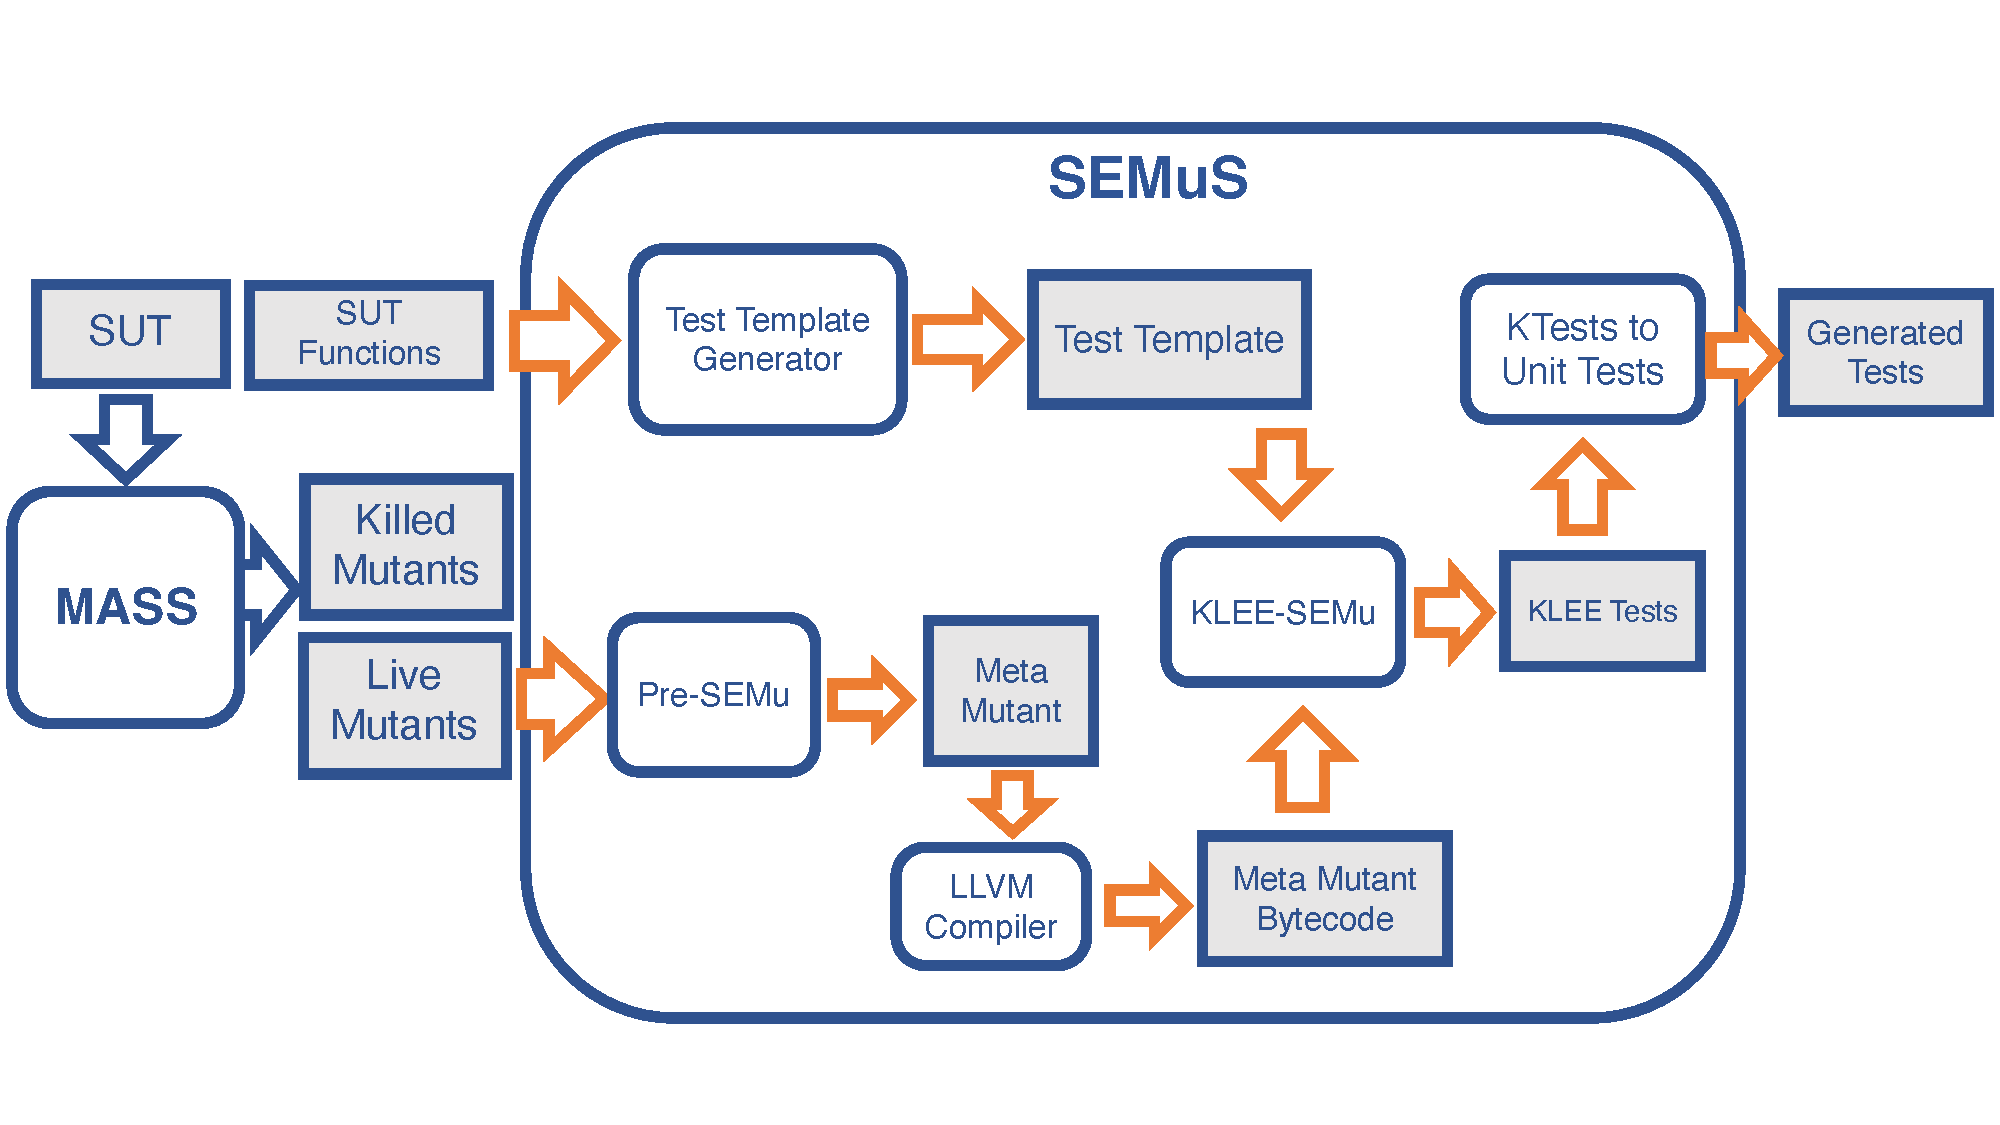
\includegraphics[width=0.8\textwidth]{images/semus-architecture}
\caption{FAQAS-SEMuS Architecture and Workflow}
\label{fig:semus_architecture}
\end{center}
\end{figure}

Figure~\ref{fig:semus_architecture} shows the architecture of SEMuS and how it interacts with MASS.

%SEMuS receives the following inputs: (a) the list of live mutants (produced by MASS), (b) the SUT, and (c) the SUT functions. 

As shown in Figure~\ref{fig:semus_architecture} SEMus is composed by five components, which are \emph{Test Template Generator},  \emph{Pre-SEMu},  \emph{KLEE-SEMu},  \emph{KTest to Unit Test}, and \emph{LLVM}.

\DONE{Why the following listing appears here? Can't we put it top or bottom?}
% !TEX root =  ../MAIN.tex

\begin{lstlisting}[style=CStyle, caption=SEMuS test template., label=test_template]
int main(int argc, char** argv) {
    // Declare variable to hold function returned value
    _Bool result_faqas_semu; 
    // Declare arguments and make input ones symbolic
    unsigned long pVal;
    int pErrCode;
    klee_make_symbolic(&pVal, sizeof(pVal), "pVal"); // Call function under test
    result_faqas_semu = T_INT_IsConstraintValid(&pVal, &pErrCode); // Make some output
    printf("FAQAS-SEMU-TEST_OUTPUT: %d\n", pErrCode);
    printf("FAQAS-SEMU-TEST_OUTPUT: %d\n", result_faqas_semu);
    return (int)result_faqas_semu;
}

\end{lstlisting}


\begin{lstlisting}[language={}, caption=Klee-test output, label=ktest]
ktest file : 'test000001.ktest'
args       : ['/MakeSym-TestGen-Input/direct/T_INT_IsConstraintValid/test.MetaMu.bc']
num objects: 2
object    0: name: b'model_version'
object    0: size: 4
object    0: data: b'\x01\x00\x00\x00'
object    1: name: b'pVal'
object    1: size: 8
object    1: data: b'\x00\x00\x00\x00\x00\x00\x00\x00'
\end{lstlisting}

\DONE{You need to provide the idea behind SEMus, that is, what it does at a high level. You need to say that the objective is to generate automatically a test template including symbolic variables and ...}

SEMuS provides the necessary components to make SEMu, and more specifically KLEE, compatible with our case studies. In particular, SEMuS (1) automates the generation of a test template including symbolic variables that guides the generation of test inputs, and (2) compiles the test template and the mutant into the format required by SEMu (i.e., LLVM IR). 


The \emph{Test Template Generator} (TTG) component automates the generation of templates for the symbolic execution search. The component receives as inputs the SUT source code and the list of SUT functions. 
Listing~\ref{test_template} shows an example of a test template generated by the TTG. The TTG generates a template for every SUT function; as shown in Listing~\ref{test_template} the component parses the function arguments and declares them symbolic through use of the KLEE function \texttt{klee\_make\_symbolic}. Then, it adds a call to the function under analysis with symbolic values, and it saves the output into the variable \texttt{result\_faqas\_semu}. Finally, the TTG adds a return call with the \texttt{result\_faqas\_semu} variable value.

The \emph{Pre-SEMu} component generates \INDEX{mutant schemata}; specifically, the component includes and compiles all the live mutants (i.e., MASS output) into a single bytecode file named the \emph{Meta Mutant}. At runtime, SEMu will select which mutant to consider for test generation based on a parameter. The compilation of the Meta Mutant into LLVM bitcode is supported by the \emph{LLVM} compiler infrastructure. 

\DONE{This listing should appear top or bottom, no?}
% !TEX root =  ../MAIN.tex
\begin{lstlisting}[float=t, language={}, caption=Klee-test output, label=ktest]
ktest file : 'test000001.ktest'
args       : ['/MakeSym-TestGen-Input/direct/T_INT_IsConstraintValid/test.MetaMu.bc']
num objects: 2
object    0: name: b'model_version'
object    0: size: 4
object    0: data: b'\x01\x00\x00\x00'
object    1: name: b'pVal'
object    1: size: 8
object    1: data: b'\x00\x00\x00\x00\x00\x00\x00\x00'
\end{lstlisting}

\emph{KLEE-SEMu} is the underlying test generation component, previously described in Section~\ref{klee-semu}. This component receives as inputs the \emph{LLVM bitcode Meta Mutant} and the \emph{Test Template} for the function under test, and proceeds to apply dynamic symbolic execution to generate test inputs to kill the mutants. The output of this component are the \emph{KLEE tests}.

% \TODO{you need to list what are "the parameters of the execution"}
A KLEE test is a binary file that contains information about the execution of KLEE such as the entry point of the analysis, and the generated test inputs.

\DONE{I fixed the following. You always have first to describe the structure of the listing and then explain its content}
An example of a KLEE test is presented in Listing~\ref{ktest}. The field \emph{args} report the entry point of the analysis; in this case, the test generation was performed for live mutants present in the function \texttt{T\_INT\_IsConstraintValid}, which SEMuS stores in a dedicated folder. The fields named \emph{object} provide information about the outputs generated by KLEE (e.g., the generated test inputs). 
For each object, the KLEE test provides a \emph{name} (usually the name of the symbolic variable), its \emph{size}, and the actual \emph{value} generated by KLEE through constraint solving (usually this is reported in binary form).
Objects are numbered. Object number \emph{0} reports information about the data structure used by KLEE, that is, the version of the structure. The other objects report information about the generated test inputs.
Our example shows that one value of size 8 was generated for the variable \texttt{pVal}, the data field shows the binary representation of the \texttt{pVal} variable, in this case \texttt{pVal=0}.


% !TEX root =  ../MAIN.tex

\begin{lstlisting}[float=t, style=CStyle,  caption=Generated test case, label=gen_test_case]
#include <stdio.h>
#include <string.h>

#include "asn1crt.c"
#include "asn1crt_encoding.c"
#include "asn1crt_encoding_uper.c"


int main(int argc, char** argv)
{
    (void)argc;
    (void)argv;

    // Declare variable to hold function returned value
    _Bool result_faqas_semu;

    // Declare arguments and make input ones symbolic
    unsigned long pVal;
    int pErrCode;
    memset(&pVal, 0, sizeof(pVal));
    const unsigned char pVal_faqas_semu_test_data[] = {0x00, 0x00, 0x00, 0x00, 0x00, 0x00, 0x00, 0x00};
    memcpy(&pVal, pVal_faqas_semu_test_data, sizeof(pVal)); // Unsigned val is 0

    // Call function under test
    result_faqas_semu = T_INT_IsConstraintValid(&pVal, &pErrCode);

    // Make some output
    printf("FAQAS-SEMU-TEST_OUTPUT: pErrCode = %d\n", pErrCode);
    printf("FAQAS-SEMU-TEST_OUTPUT: result_faqas_semu = %d\n", result_faqas_semu);
    return (int)result_faqas_semu;
}
\end{lstlisting}

\DONE{I updated the following, please check}

The component \emph{KTest to Unit Test} (KTU) converts a KLEE test into a readable, executable C test case. Similar to the TTG component, the KTU uses a template to hold the specifics variables of each function under test. 
Listing~\ref{gen_test_case} shows an example of a test case generated for a mutant present in the function \texttt{T\_INT\_IsConstraintValid}. For instance, line 20 shows that the variable \texttt{pVal} is initially filled with 0 (to clean it), then in line 21, it is filled with the value stored in the variable \texttt{pVal\_faqas\_semu\_test\_data}, which holds the binary output produced by KLEE. In line 25, the function under test is invoked with the concrete value of \texttt{pVal}. Finally, the KTU print the function return value and the value of every variable passed by reference.
At the current stage, KTU does not generate assertions. Assertions need to be implemented by engineers in place of the generated \emph{printfs} because only the engineers can know, based on specifications, what are the values to be expected at the end of the test case execution.


\ENDCHANGEDWPT

\ENDCHANGEDFR

% \newpage
% % !TEX root = MAIN.tex
\chapter{ESA Revisions}

%% !TEX root = MAIN.tex

\section{Responses to ESA comments provided on 12.04.2021}
\label{sec:ESA:comments:1}

Comments IDs appear also in the main document next to the text modified to address the comment. To save space in the main text, the prefix \emph{ITSR-SSS-PABG-} has been abbreviated as \emph{P-}.

\setlength\LTleft{0pt}
\setlength\LTright{0pt}
\tiny 
%@{\extracolsep{\fill}}
\begin{longtable}{|p{1.5cm}|p{12cm}|@{}}
%\caption{\normalsize .}
%\label{table:comments:responses} 
\textbf{Comment ID}&\textbf{Response}\\
\\
\hline
P-1&
\begin{minipage}{12cm}
We will need to discuss the detail of the merge of the two specifications during the review meeting.
\end{minipage}\\
\\
\hline

P-2&
\begin{minipage}{12cm}
Done.
\end{minipage}\\
\\
\hline

P-3&
\begin{minipage}{12cm}
Done.
\end{minipage}\\
\\
\hline

P-4&
\begin{minipage}{12cm}
Done.
\end{minipage}\\
\\
\hline

P-5&
\begin{minipage}{12cm}
Done.
\end{minipage}\\
\\
\hline

P-6&
\begin{minipage}{12cm}
Done.
\end{minipage}\\
\\
\hline

P-7&
\begin{minipage}{12cm}
Done.
\end{minipage}\\
\\
\hline

P-8&
\begin{minipage}{12cm}
Done.
\end{minipage}\\
\\
\hline

P-9&
\begin{minipage}{12cm}
It is worth discussing if it makes sense to perform mutation analysis without code coverage.
\end{minipage}\\
\\
\hline


P-10&
\begin{minipage}{12cm}
We always generate all the mutants because it's fast. End-users have the option to execute a subset of them.
\end{minipage}\\
\\
\hline

P-11&
\begin{minipage}{12cm}
We changed a sentence, but this requirement is long because we had to provide an explanation missing from D2.
\end{minipage}\\
\\
\hline

P-12&
\begin{minipage}{12cm}
\end{minipage}\\
\\
\hline

P-13&
\begin{minipage}{12cm}
\end{minipage}\\
See P-8\\
\hline

P-14&
\begin{minipage}{12cm}
\end{minipage}\\
Action item. To be done for the end of WP3.\\
\hline


P-15&
\begin{minipage}{12cm}
TOD
\end{minipage}\\
\hline

P-16&
\begin{minipage}{12cm}
Done.
\end{minipage}\\
\hline

P-17&
\begin{minipage}{12cm}
We will provide a table for end of WP3.
\end{minipage}\\
\hline
                                                
\end{longtable}
\normalsize

\clearpage

% !TEX root = MutationTestingSurvey.tex

\section{Responses to ESA comments provided on 03.04.2020}
\label{sec:ESA:comments:2}


\setlength\LTleft{0pt}
\setlength\LTright{0pt}
\tiny 
\begin{longtable}{|p{1.5cm}|p{12cm}|@{}}
\label{table:comments:responses} 
\textbf{Comment ID}&\textbf{Comment and Response (below)}\\
\\
\midrule
C6 \& C7
&
Have you seen numbers for this mutation score and threshold in the literature? Is this something to be checked during the use case evaluation?
\\
\cmidrule{2-2}
&
We have addressed the comments above.
\TODO{OScar: please check if the survey of Papadakis say something aboth teh threshold (C7)}
\\
\hline
C8
&
Elaborate a bit more on C8 (pros and cons of doing mutation at source code / IR/ Assembly/ Executable);
\\
\cmidrule{2-2}
&
\TODO{Oscar: you may refer to taht paper of Darko Marinov and Co. to say IR is not good}
\\
\hline
C31
&
What is this sufficient set of operators?
\\
\cmidrule{2-2}
&
\TODO{Oscar}
\\
\hline
C32
&
Can you please add the solution for this example? i.e. do we need two different test cases of isPalindrome to detect both mutants?
\\
\cmidrule{2-2}
&
\TODO{Oscar}
\\
\hline
C33
&
Even if the objectives are complementary, both of them should be pursued for a data mutation testing approach?
\\
\cmidrule{2-2}
&
We have addressed the comment above.
\\
\hline
C34
&
The sentence sounds weird... To automate?? Is this activity something that can be automated?
\\
\cmidrule{2-2}
&
We have addressed the comment above by clarifying our text.
\\
\hline
C35
&
Is it possible to add an example of equivalent and redundant mutants?
\\
\cmidrule{2-2}
&
We have added the requested examples.
\\
\hline
C36
&
\begin{minipage}{12cm}
Related to automation, in my opinion, what it is key is that the test assessment process (for both data and code mutation) is as much automated as possible.\\

Automated generation of test cases is a very nice to have. In an industrial environment, let's say that we could afford spending some time to manually augment the test suite.\\

You may consider this to prioritize tasks within this activity.
\end{minipage}
\\
\cmidrule{2-2}
&
We agree on the comment. No need to change the text in this deliverable.
\\
\hline
C37
&
Are we missing a chapter to address the Generation of Test Oracles?\\
\cmidrule{2-2}
&
We have added a section concerning generation of test oracles for code-driven mutation testing (Section~\ref{sec:oraclesGeneration:codeDriven}) and data-driven mutation testing 
(Section~\ref{sec:oracles:dataMutation}).
\\
\hline
C38
&
\begin{minipage}{12cm}
a. From these Case Studies, is there any that you would like to try out within FAQAS?\\

b. One thing that we may need for FAQAS framework is to have kind of a test suite allowing to test the tool, and also to test the tool when new versions will be produced. Would any of these case studies fulfill that?
\end{minipage}
\\
\cmidrule{2-2}
&
We have discussed this topics by voice.
\\
\hline
C39
&
Do you have any information on the kind of test suite? (e.g. is it unit testing, system testing, ...)
\\
\cmidrule{2-2}
&
\TODO{}
\\
\hline
C40
&
Are these case studies focused on Code-Mutation, Data-Mutation, or both?\\
\cmidrule{2-2}
&
\TODO{}
\\
\hline
C41
&
Is there any meaningful conclusion (positive or negative) from those industrial case studies?\\
\cmidrule{2-2}
&
\TODO{}
\\
\hline
C42
&
\begin{minipage}{12cm}
Can we make a conclusion paragraph on this?\\

e.g. No tool based on mutation testing is known to be used within an industrial software development environment\\
e.g. Mutation testing is seen applied mainly within research environments\\
etc, etc
\end{minipage}
\\
\cmidrule{2-2}
&
\TODO{}
\\
\hline
C43
&
Is there any of these trends that could be meaningful to explore?
\\
\cmidrule{2-2}
&
\TODO{}
\\
\hline
C44
&
\begin{minipage}{12cm}
	\begin{itemize}
		\item Is there any particular trend for Code-Based mutation testing? (e.g. research is on-going or vanishing, the way to apply it, the type of operators used, the tools supporting it, ...)
		\item Any particular trend for Data-Based mutation testing?
	\end{itemize}
\end{minipage}
\\
\cmidrule{2-2}
&
\TODO{}
\\
\hline
C45&
\begin{minipage}{12cm}
D1 is fulfilling well requirement R1-1 as in the SoW. There is only one exception, on the red sentence below:\\

[R1-1.c] The applications of mutation testing (e.g. code and data mutation, test-suite evaluation, test cases generation, test-data generation, \textcolor{red}{code quality improvement}, ...)\\

The evaluation of code quality improvement is to be looked at. Indeed, this would be a secondary objective of applying mutation testing on space systems, but we would like to understand if mutation testing could help improve the code quality or not.\\
\end{minipage}
\\
\cmidrule{2-2}
&
\begin{minipage}{12cm}
We added a paragraph on Chapter~\ref{chapter:trends} explaining that there are no works in literature about quality code improvement based on code-driven mutation testing.
\end{minipage}
\\

\bottomrule                                                             
\end{longtable}
\normalsize

\clearpage



\clearpage

\printindex

\end{document}
